\ifdefined\pdfminorversion
\pdfminorversion=7
\fi

\documentclass[12pt,a4paper,openany]{report}

\usepackage[utf8]{inputenc}
\usepackage[T1]{fontenc}
\usepackage{times}
\usepackage{geometry}
\usepackage{setspace}
\usepackage{graphicx}
\usepackage{pdfpages}
\usepackage{array}
\usepackage{longtable}
\usepackage{ragged2e}
\usepackage{titlesec}
\usepackage{caption}
\usepackage[hidelinks]{hyperref}
\usepackage{float}

\hypersetup{
    pdftitle={Conception d'une solution data-driven pour le suivi et l'analyse des operations de merchandising terrain du projet Unilever chez Smollan Morocco},
    pdfauthor={Hamza CHARMAQE}
}

\geometry{
    left=2.5cm,
    right=2.5cm,
    top=2.5cm,
    bottom=2.5cm
}

\graphicspath{
    {figures/}
    {figures/architecture/}
    {figures/dashboards/}
    {figures/database/}
    {figures/etl/}
    {figures/mobile/}
    {figures/validation/}
}

\setlength{\parindent}{1.25cm}
\setlength{\parskip}{6pt}
\setlength{\emergencystretch}{3em}
\setstretch{1.15}
\justifying

\setcounter{secnumdepth}{3}
\setcounter{tocdepth}{3}

\pagestyle{headings}

\titleformat{\chapter}[hang]
{\normalfont\fontsize{16}{19.2}\bfseries}
{\MakeUppercase{\chaptername\ \thechapter\ :}}{0.6em}
{\MakeUppercase}
\titlespacing*{\chapter}{0pt}{0pt}{28pt}

\renewcommand{\thesection}{\Roman{section}.}
\renewcommand{\thesubsection}{\Roman{section}.\arabic{subsection}}
\renewcommand{\thesubsubsection}{\Roman{section}.\arabic{subsection}.\arabic{subsubsection}}

\titleformat{\section}
{\normalfont\fontsize{14}{16.8}\bfseries}
{\thesection}{1em}{}
\titlespacing*{\section}{0pt}{14pt}{8pt}

\titleformat{\subsection}
{\normalfont\fontsize{12}{14.4}\bfseries}
{\thesubsection}{1em}{}
\titlespacing*{\subsection}{0pt}{10pt}{6pt}

\titleformat{\subsubsection}
{\normalfont\fontsize{12}{14.4}\bfseries}
{\thesubsubsection}{1em}{}
\titlespacing*{\subsubsection}{0pt}{8pt}{4pt}

\captionsetup{
    font={footnotesize,it},
    labelfont={footnotesize,it},
    justification=centering,
    labelsep=space,
    skip=6pt
}

\renewcommand{\contentsname}{Table des matieres}
\renewcommand{\listfigurename}{Liste des figures}
\renewcommand{\listtablename}{Liste des tableaux}
\renewcommand{\chaptername}{Chapitre}
\renewcommand{\figurename}{Figure}
\renewcommand{\tablename}{Tableau}
\renewcommand{\chaptermark}[1]{\markboth{Chapitre \thechapter{} : #1}{}}
\let\cleardoublepage\clearpage

\begin{document}

\hypersetup{pageanchor=false}

\includepdf[pages=1,pagecommand={\thispagestyle{empty}}]{cover_page.pdf}
\hypersetup{pageanchor=true}

\clearpage
\pagenumbering{roman}
\chapter*{Dédicaces}
\addcontentsline{toc}{chapter}{Dédicaces}

Je dédie ce travail à mes chers parents, pour leur soutien, leurs sacrifices et leur confiance tout au long de mon parcours académique. Leur encouragement permanent a constitué une source essentielle de motivation et de persévérance.

Je le dédie également à ma famille, à mes proches et à toutes les personnes qui m’ont accompagné, conseillé ou soutenu durant cette période de formation et de stage.

Enfin, je dédie ce mémoire à l’ensemble des enseignants et encadrants qui ont contribué à ma formation et à mon développement personnel et professionnel.

\clearpage
\phantomsection
\markboth{REMERCIEMENTS}{}
\thispagestyle{frontmatterstyle}

\FrontTitlePersonal{Remerciements}

\begin{center}
\begin{minipage}{0.78\textwidth}
\justifying
\setlength{\parindent}{0.7cm}
\setlength{\parskip}{11pt}

Je remercie avant tout Allah, qui m’a donné la force, la patience et la volonté nécessaires pour mener à bien ce Projet de Fin d’Études.

J’adresse mes sincères remerciements à mes parents, pour leur soutien permanent, leurs sacrifices et leur confiance tout au long de mon parcours académique. Leur présence a toujours été une source essentielle de motivation.

Je tiens à exprimer ma gratitude à mon encadrant professionnel, \textbf{M. Aissa Ahlali}, pour son accompagnement, sa disponibilité et ses orientations tout au long de mon stage au sein de Smollan Morocco.

Je remercie également mon encadrant académique, \textbf{Pr. Hicham Moutachaouik}, pour son suivi, ses conseils et ses remarques constructives tout au long de la réalisation de ce travail. J’adresse aussi mes remerciements aux membres du jury, \textbf{Pr. Serkaite} et \textbf{Pr. Kanouss}, pour le temps consacré à l’évaluation de ce travail, ainsi que pour leurs remarques et recommandations.

Enfin, je remercie l’ensemble des collaborateurs de Smollan Morocco avec lesquels j’ai eu l’occasion d’échanger, ainsi que toutes les personnes qui m’ont soutenu de près ou de loin durant cette période.

\end{minipage}
\end{center}

\clearpage
\chapter*{Resume}
\addcontentsline{toc}{chapter}{Resume}

% TODO: Rediger le resume final en francais apres stabilisation du contenu du rapport.

\textbf{Mots-cles :} % TODO: Ajouter les mots-cles finaux.


\clearpage
\phantomsection
\markboth{ABSTRACT}{}
\thispagestyle{frontmatterstyle}

\FrontTitleSummary{Abstract}

\begin{FrontTextBlock}
This final-year project focuses on the design of a data\mbox{-}driven solution for monitoring and analyzing Unilever field merchandising operations at Smollan Morocco. The project starts from an initial process that strongly depends on \textit{Data Dump} and \textit{Coverage} exports, Excel-based processing, and separately prepared reports.

The proposed solution centralizes the data in a MySQL database through a Data Engineering pipeline, then makes it available through Power BI dashboards, a client-side mobile consultation application, and an internal back-office portal. A business validation engine also identifies situations requiring internal review, especially through OSA and GPS control rules.

The obtained results show improved traceability, reduced data preparation time, and a more structured use of field execution data. The project therefore provides a functional foundation for strengthening operational monitoring and merchandising data analysis in a real professional context.

\vspace{0.8cm}

\noindent\textbf{Keywords:} Data Engineering, ETL, MySQL, field merchandising, OSA, GPS, Power BI, mobile application, back-office, business validation.
\end{FrontTextBlock}
\clearpage
\tableofcontents
\clearpage
\listoffigures
\clearpage
\listoftables
\clearpage
\chapter*{Liste des abréviations}
\markboth{LISTE DES ABRÉVIATIONS}{}
\addcontentsline{toc}{chapter}{Liste des abréviations}

\vspace{0.5cm}

\begin{center}
\begin{minipage}{0.82\textwidth}

\renewcommand{\arraystretch}{1.25}
\setlength{\tabcolsep}{6pt}

\begin{tabularx}{\textwidth}{>{\bfseries}p{2.6cm} X}
\toprule
\textbf{Abréviation} & \textbf{Signification} \\
\midrule
PFE & Projet de Fin d’Études. \\
GT & General Trade. \\
MT & Modern Trade. \\
Adhoc & Visite non planifiée, réalisée hors du planning initial. \\
OSA & On Shelf Availability. \\
GPS & Global Positioning System. \\
SOS & Share of Shelf. \\
SKU & Stock Keeping Unit. \\
KPI & Key Performance Indicator. \\
BI & Business Intelligence. \\
CSV & Comma-Separated Values. \\
ETL & Extract, Transform, Load. \\
DB & Database. \\
DTO & Data Transfer Object. \\
MySQL & Système de gestion de base de données relationnelle. \\
SQL & Structured Query Language. \\
API & Application Programming Interface. \\
HTTP & HyperText Transfer Protocol. \\
JSON & JavaScript Object Notation. \\
REST & Representational State Transfer. \\
UML & Unified Modeling Language. \\
URL & Uniform Resource Locator. \\
\bottomrule
\end{tabularx}

\end{minipage}
\end{center}
\clearpage

\pagenumbering{arabic}

\chapter*{Introduction générale}
\markboth{INTRODUCTION GÉNÉRALE}{}
\addcontentsline{toc}{chapter}{Introduction générale}

Dans le secteur des biens de grande consommation, la performance commerciale ne dépend pas uniquement de la disponibilité des produits dans les entrepôts ou dans les circuits de distribution. Elle dépend aussi de la qualité de l’exécution réalisée en magasin. La présence effective des produits en rayon, le respect des standards de merchandising, la visibilité des marques, la conformité du placement et la fiabilité des informations remontées depuis le terrain constituent des éléments essentiels pour piloter l’activité commerciale et accompagner la prise de décision.

Dans ce contexte, les données issues des opérations terrain occupent une place importante. Elles permettent de suivre l’activité des merchandisers, d’évaluer la couverture des points de vente, de contrôler la disponibilité des produits, d’identifier les écarts d’exécution et de produire des indicateurs destinés aux équipes internes ainsi qu’au client. Cependant, lorsque ces données sont exploitées quotidiennement à travers plusieurs fichiers Excel, rapports séparés et traitements manuels, leur utilisation devient plus lourde, moins centralisée et plus difficile à suivre dans le temps.

Le présent projet de fin d’études s’inscrit dans le cadre d’un stage réalisé au sein de Smollan Morocco, en tant que Data Analyst Intern, autour du projet Unilever. Dans ce projet, les merchandisers effectuent leurs visites en magasin à travers l’application mobile Smart 3. Les données collectées sont ensuite synchronisées vers le portail Smollan, à partir duquel les équipes opérationnelles exportent principalement deux fichiers : \textit{Data Dump} et \textit{Coverage}. Ces fichiers constituent la base du suivi quotidien, puisqu’ils alimentent les rapports de couverture, de déviation, de disponibilité produit, de qualité d’exécution, de planogramme, de placement et d’autres indicateurs liés au merchandising terrain.

L’exploitation de ces fichiers répond à un besoin opérationnel réel, mais elle présente aussi plusieurs limites. Les données sont dispersées entre plusieurs exports, les traitements sont répétés, l’historique reste difficile à consolider et certaines vérifications nécessitent encore des analyses manuelles. Cette situation peut ralentir la préparation des rapports et compliquer l’identification rapide des situations nécessitant une attention particulière, notamment lorsqu’il s’agit de croiser les informations de couverture, les réponses terrain et les indicateurs métier.

Le sujet de ce PFE porte donc sur la conception d’une solution data-driven pour le suivi et l’analyse des opérations de merchandising terrain du projet Unilever chez Smollan Morocco. L’objectif n’est pas de remplacer totalement les outils existants, mais de proposer une approche complémentaire permettant de mieux structurer les données, d’automatiser une partie des traitements, de centraliser l’historique, d’appliquer des règles de validation métier et de restituer les résultats à travers des supports adaptés aux différents usages.

La solution proposée s’appuie sur une chaîne de traitement des données permettant d’exploiter les fichiers \textit{Data Dump} et \textit{Coverage}, de les transformer et de les charger dans une base MySQL centralisée. Cette base constitue le socle de la solution. Elle alimente ensuite plusieurs composantes : un moteur de validation destiné à produire des signaux de contrôle internes, des services backend permettant d’exposer les données selon les usages, des tableaux de bord Power BI pour l’analyse décisionnelle, une application mobile de consultation côté client et un portail back-office réservé au suivi interne des situations détectées.

La démarche adoptée repose d’abord sur la compréhension du processus métier existant, depuis la visite effectuée par le merchandiser jusqu’à l’exploitation des données par les équipes internes. Elle se poursuit par l’analyse des sources de données, la conception d’une architecture adaptée, le développement du pipeline Data Engineering, la structuration de la base relationnelle, la mise en place des règles de validation et le développement des couches de restitution. Cette progression permet de relier les choix techniques aux besoins opérationnels observés durant le stage.

Le rapport est structuré selon la progression du projet. Il commence par la présentation du contexte général, de l’organisme d’accueil et de la problématique traitée. Il analyse ensuite l’existant et les besoins identifiés, avant de présenter la conception globale de la solution retenue. Les chapitres suivants décrivent la mise en place des principales composantes techniques et applicatives, puis évaluent les résultats obtenus, les apports du projet et les limites de la solution réalisée.
\chapter{Contexte général du projet}

\section{Introduction}

Ce premier chapitre présente le cadre général dans lequel s’inscrit le Projet de Fin d’Études réalisé au sein de Smollan Morocco. Il introduit l’organisme d’accueil, le client concerné par le projet, ainsi que le contexte métier lié aux opérations de merchandising terrain.

Il permet également de préciser la problématique identifiée, les objectifs poursuivis par le projet et la méthodologie de travail adoptée durant le stage. Ce chapitre constitue ainsi une étape de cadrage essentielle avant l’analyse de l’existant et la conception de la solution proposée.

\section{Présentation de l’organisme d’accueil}

\subsection{Présentation générale de Smollan}

Smollan est un groupe international spécialisé dans les solutions de croissance retail et d’exécution commerciale au point de vente. Son rôle consiste à accompagner les marques et les distributeurs dans l’amélioration de leur performance commerciale, en combinant présence terrain, activation de marque, suivi de l’exécution et exploitation des données opérationnelles.

L’activité de Smollan ne se limite pas au merchandising. Elle couvre plusieurs dimensions complémentaires, notamment le \textit{Sales \& Merchandising}, l’\textit{Activation \& Experience}, les solutions \textit{Data \& Technology} ainsi que des services liés au commerce digital. Cette diversité permet à l’entreprise d’intervenir sur différents niveaux de la chaîne retail : exécution en magasin, visibilité des produits, expérience consommateur, reporting, analyse de performance et aide à la décision.

Dans le cadre du stage, Smollan Morocco constitue l’organisme d’accueil au sein duquel le projet a été réalisé. Le travail s’inscrit dans un contexte de digitalisation et de valorisation des données terrain, avec pour objectif d’améliorer le suivi et l’analyse des opérations liées au projet Unilever.

La figure suivante présente le logo de l’organisme d’accueil.

\begin{figure}[H]
    \centering
    
\includegraphics[width=0.45\textwidth]{SMOLLAN.png}
    \caption{Logo de Smollan}
    \label{fig:logo-smollan}
\end{figure}

Ce logo permet d’identifier l’organisme d’accueil dans lequel s’inscrit le projet et introduit le contexte professionnel du stage.

\subsection{Domaines d’activité de Smollan}

Les domaines d’activité de Smollan s’articulent autour de plusieurs services complémentaires destinés à améliorer la performance des marques dans l’environnement retail. Ils couvrent notamment l’exécution commerciale en point de vente, l’activation et l’expérience consommateur, ainsi que l’exploitation des données et des technologies pour le suivi et l’analyse de la performance.

La figure suivante propose une synthèse des principaux domaines d’activité de Smollan.

\begin{figure}[H]
    \centering
    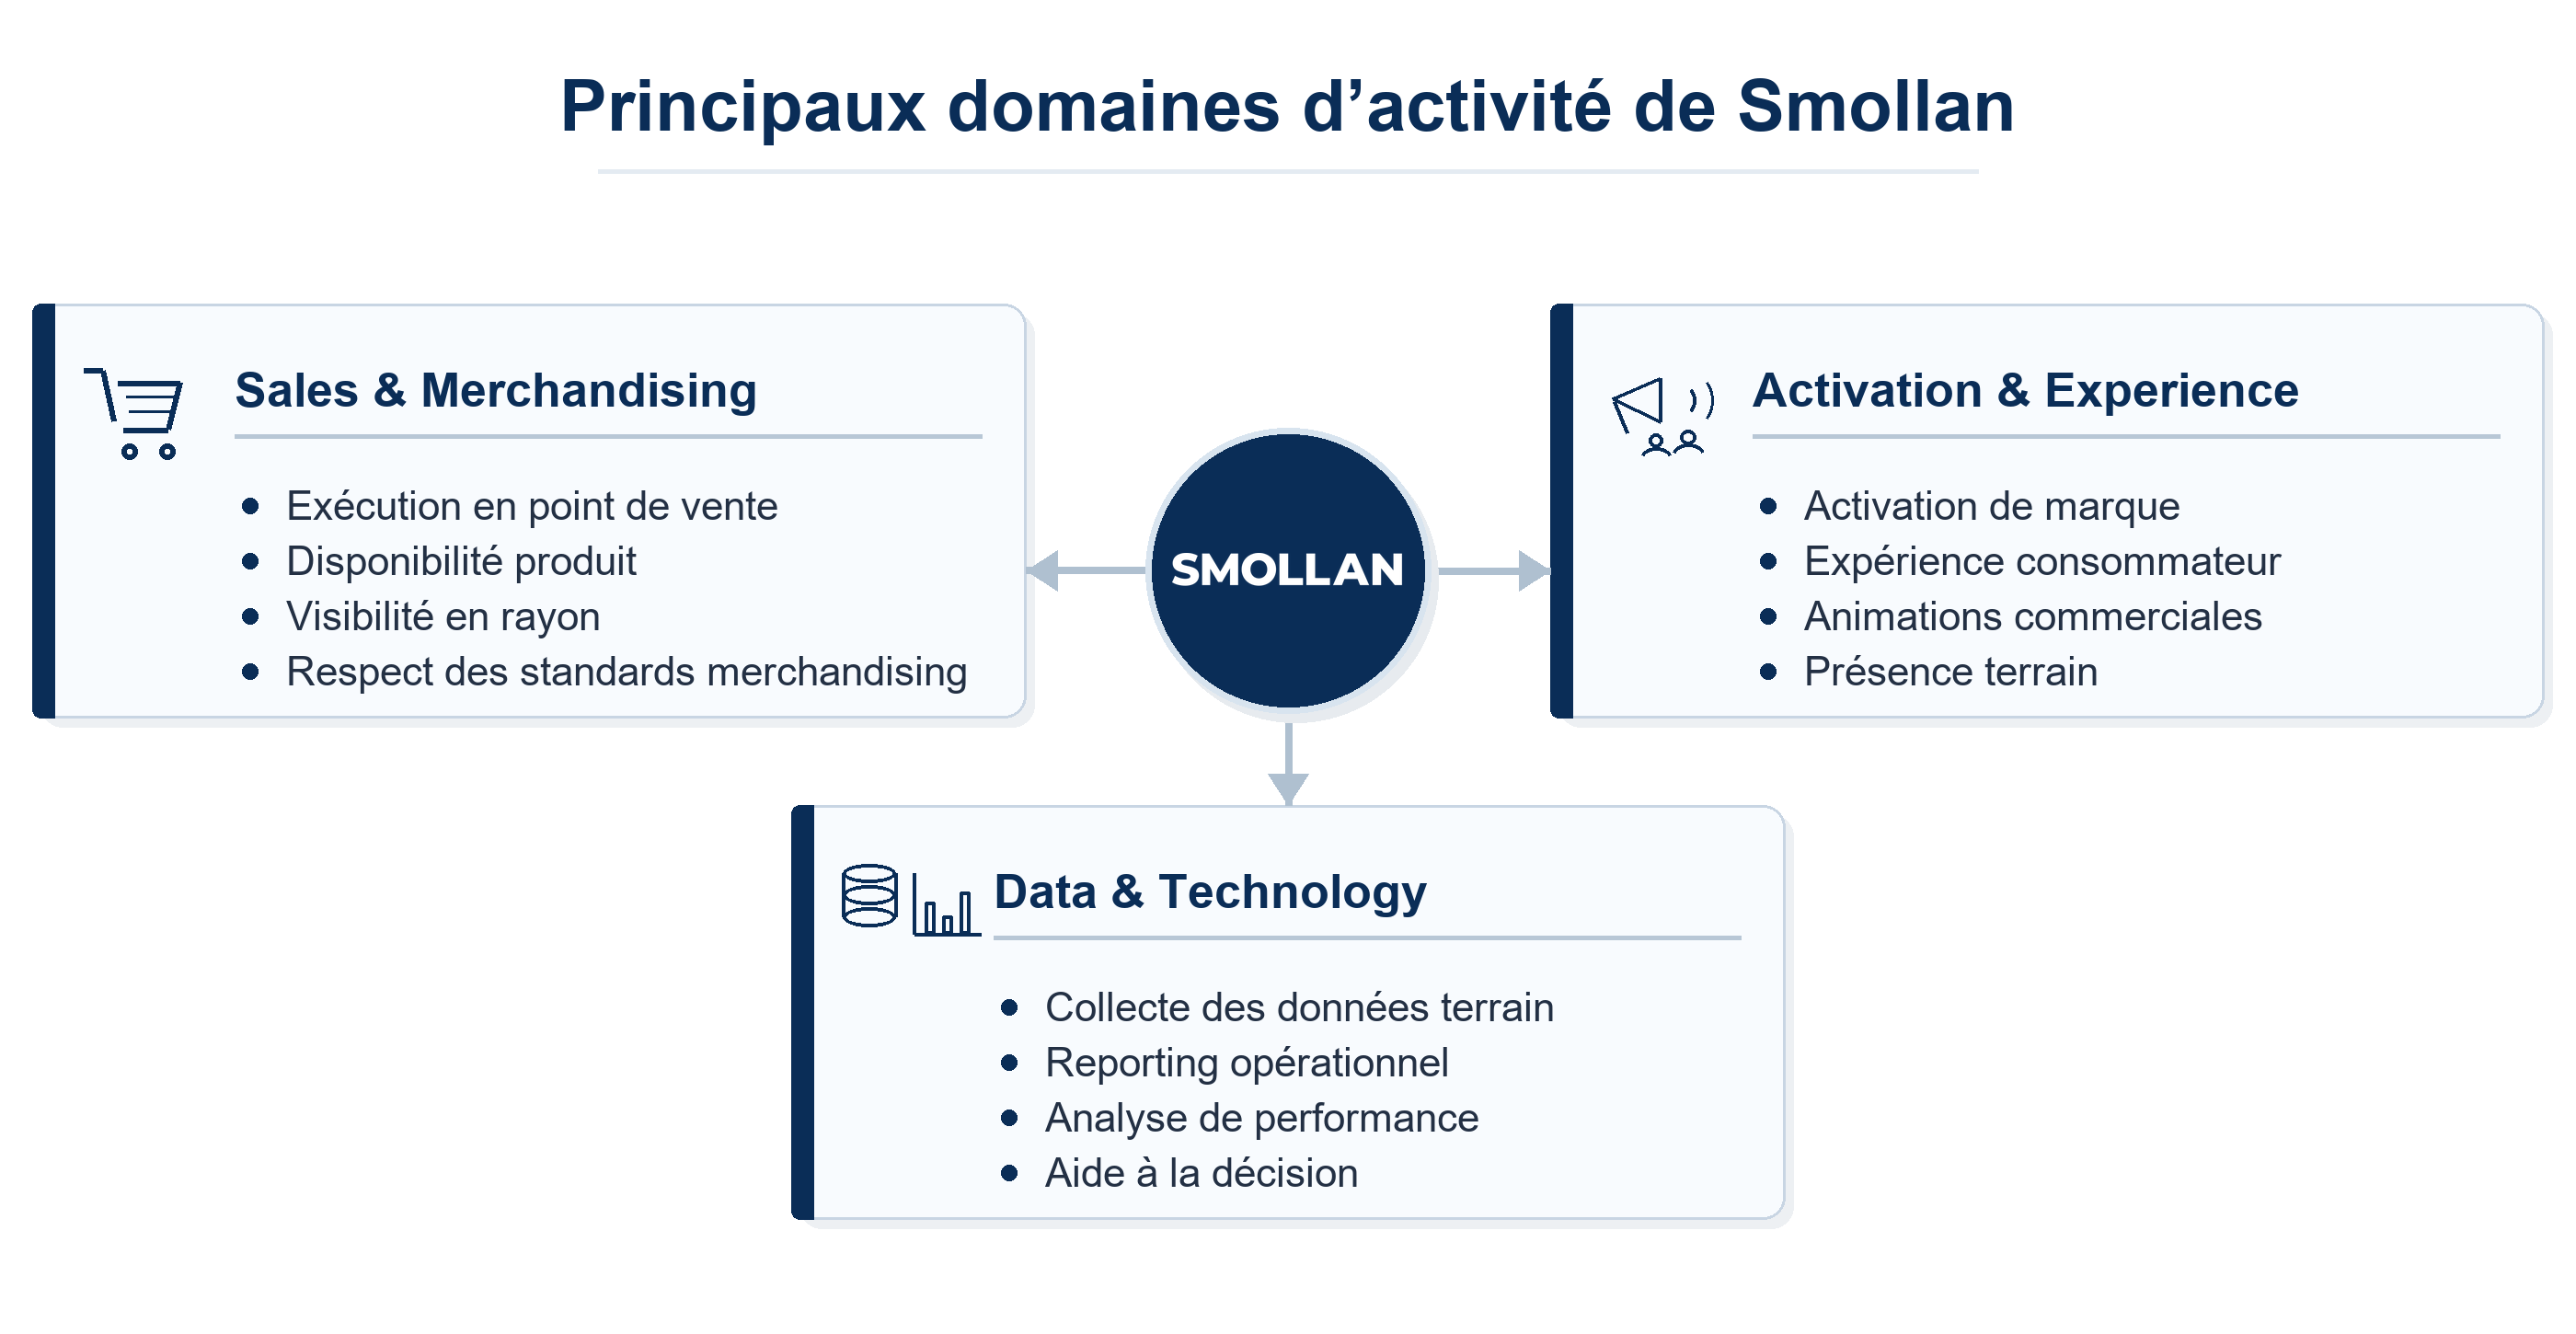
\includegraphics[width=\textwidth]{figures/architecture/smollan_activity_areas.png}
    \caption{Principaux domaines d’activité de Smollan}
    \label{fig:smollan-activity-areas}
\end{figure}

Ces domaines montrent que Smollan intervient à la fois dans l’exécution commerciale, l’activation des marques, la collecte d’informations terrain et l’analyse de la performance. Cette orientation explique le lien direct entre le contexte métier du stage et la mise en place d’une solution data-driven pour le suivi des activités terrain.

\subsection{Principaux clients et partenaires de Smollan}

Smollan accompagne différents types de marques, de distributeurs et de partenaires opérant dans des environnements commerciaux variés. Ces collaborations peuvent concerner les biens de grande consommation, les boissons, l’hygiène et les soins, la technologie, le retail ou encore l’agroalimentaire. L’objectif n’est pas de présenter une liste exhaustive de partenaires, mais de situer l’écosystème dans lequel les activités de Smollan s’inscrivent.

Dans le cadre de ce Projet de Fin d’Études, le périmètre étudié est centré sur les opérations de merchandising terrain liées au projet Unilever. Cette précision permet de distinguer l’écosystème général de Smollan du champ d’analyse réellement traité dans le rapport.

La figure suivante illustre l’écosystème général dans lequel s’inscrivent les activités de Smollan.

\begin{figure}[H]
    \centering
    
\includegraphics[width=0.45\textwidth]{SMOLLAN.png}
    \caption{Illustration de l’écosystème de partenaires et clients de Smollan}
    \label{fig:smollan-partners}
\end{figure}

Cette illustration accompagne la présentation de l’écosystème de Smollan, qui couvre différents secteurs d’activité et différents types de partenaires. Dans le cadre du présent rapport, le périmètre d’étude reste toutefois centré sur les opérations de merchandising liées au projet Unilever.

\subsection{Smollan Morocco}

Smollan Morocco représente la présence locale du groupe Smollan au Maroc. Elle accompagne plusieurs clients dans le suivi de leurs activités commerciales et merchandising, en s’appuyant sur des équipes terrain, des superviseurs et des outils de reporting opérationnel.

Dans ce contexte, les données collectées sur le terrain jouent un rôle important dans le pilotage quotidien des opérations. Elles permettent de suivre l’exécution des visites, la couverture des magasins, la disponibilité des produits, la qualité d’exécution et les indicateurs nécessaires à la prise de décision.

Le projet réalisé durant le stage s’intègre dans cette logique. Il vise à mieux exploiter les données issues du terrain afin de renforcer le suivi opérationnel, de structurer l’historique des informations et de proposer des supports de restitution adaptés aux différents utilisateurs.

\section{Présentation du client Unilever}

Unilever est une entreprise internationale opérant dans le secteur des biens de grande consommation. Ses activités couvrent plusieurs catégories de produits, notamment les soins personnels, l’hygiène, l’entretien de la maison, l’alimentation et d’autres produits utilisés quotidiennement par les consommateurs.

Dans le cadre des opérations de merchandising, Unilever accorde une importance particulière à la disponibilité de ses produits en magasin, à leur visibilité en rayon, au respect des standards d’exécution et à la qualité de la présence de ses marques dans les points de vente. Ces éléments sont essentiels pour soutenir la performance commerciale et assurer une meilleure expérience d’achat.

Le projet réalisé chez Smollan Morocco concerne le suivi des opérations de merchandising terrain liées au projet Unilever. Il vise à améliorer l’exploitation des données collectées en magasin afin de faciliter le pilotage, l’analyse et la consultation des informations d’exécution.

La figure suivante présente le logo du client concerné par le projet.

\begin{figure}[H]
    \centering
    
\includegraphics[width=0.28\textwidth]{Logo-blue-transparent-RGB.eps}
    \caption{Logo d’Unilever}
    \label{fig:logo-unilever}
\end{figure}

La présence du logo permet d’identifier le client autour duquel s’articulent les opérations de merchandising étudiées dans ce projet.

\section{Contexte métier du merchandising terrain}

Le merchandising terrain regroupe l’ensemble des actions réalisées en point de vente afin d’assurer la disponibilité, la visibilité et la bonne présentation des produits. Dans le cadre du projet Unilever, ces actions sont réalisées par des merchandisers qui effectuent des visites en magasin à l’aide de l’application Smart 3.

Lors de chaque visite, le merchandiser renseigne plusieurs informations relatives à l’exécution terrain. Ces informations peuvent concerner la disponibilité des produits, la qualité d’exécution, le respect du planogramme, le placement primaire ou secondaire, le SOS (\textit{Share of Shelf}), les relevés de prix, les photos justificatives ainsi que les données de localisation collectées par l’application.

Le suivi de ces opérations implique plusieurs niveaux d’exploitation. D’une part, les données saisies permettent d’assurer un suivi opérationnel interne, notamment pour vérifier l’avancement des visites, les écarts de couverture ou les situations nécessitant une justification. D’autre part, certaines informations sont utilisées pour préparer des reportings destinés au client, notamment autour de la disponibilité produit, de la qualité d’exécution ou de la visibilité en rayon.

Dans ce contexte, la donnée terrain devient un élément central du pilotage. Elle ne sert pas uniquement à constater qu’une visite a été réalisée, mais permet également d’analyser la qualité de l’exécution, de suivre les performances opérationnelles et d’améliorer la visibilité des différents acteurs sur l’activité en magasin.

La figure suivante présente une vue simplifiée des principaux acteurs et flux métier liés aux opérations de merchandising terrain.

\begin{figure}[H]
    \centering
    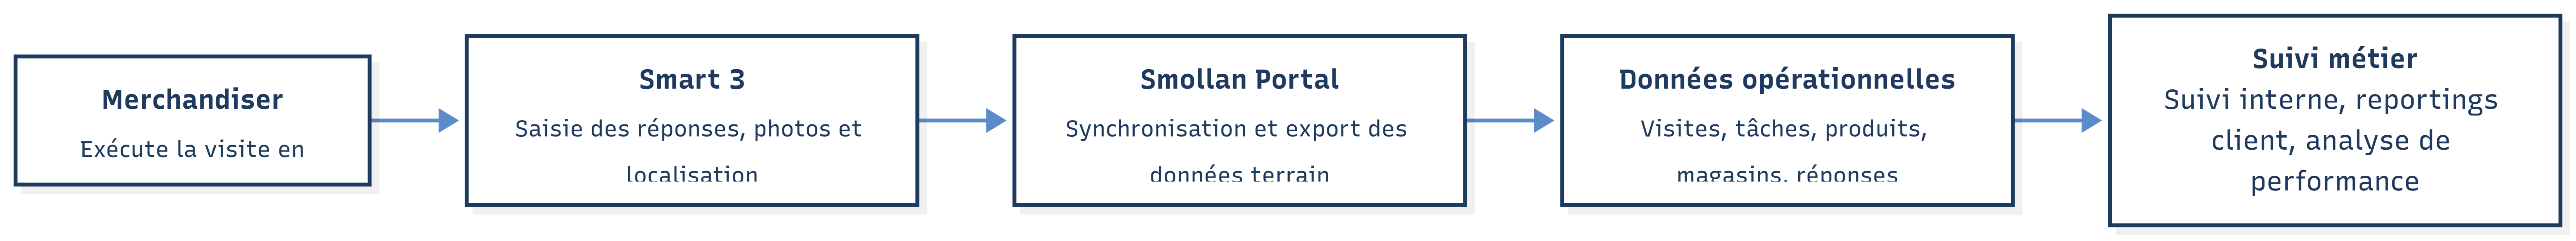
\includegraphics[width=0.9\textwidth]{figures/architecture/flux_metier_merchandising.png}
    \caption{Acteurs et flux métier des opérations de merchandising terrain}
    \label{fig:business-context-flow}
\end{figure}

Ce schéma montre que les informations collectées en magasin constituent la base du suivi opérationnel. Elles sont saisies dans l'application Smart 3, synchronisées vers le portail Smollan, puis exploitées pour alimenter le suivi interne et les reportings destinés au client.

\section{Problématique}

Le suivi des opérations terrain du projet Unilever repose sur des données collectées quotidiennement à travers l’application Smart 3, puis exportées depuis le portail Smollan sous forme de fichiers Excel. Ces fichiers contiennent une quantité importante d’informations relatives aux visites, aux magasins, aux merchandisers, aux produits et aux tâches exécutées.

Cependant, l’exploitation de ces données devient complexe lorsque les informations sont dispersées entre plusieurs fichiers et reportings. Le fichier \textit{Data Dump} apporte le détail des réponses terrain, tandis que le fichier \textit{Coverage} permet de suivre les visites planifiées, réalisées, rejetées, déviées ou non effectuées. Cette séparation nécessite un travail de structuration afin d’obtenir une vision cohérente, fiable et exploitable des opérations.

Par ailleurs, les besoins de restitution ne sont pas identiques selon les utilisateurs. Le management et les équipes internes ont besoin d’indicateurs consolidés pour le pilotage et le contrôle opérationnel, tandis que les superviseurs côté client doivent disposer d’une consultation plus ciblée sur les magasins qui leur sont affectés. Les situations nécessitant une validation ou une vérification interne doivent, quant à elles, être traitées dans un espace back-office adapté.

La problématique du projet peut donc être formulée comme suit :

\begin{quote}
Comment concevoir une solution data-driven permettant de centraliser et structurer les données de merchandising terrain du projet Unilever, afin de proposer des restitutions adaptées au pilotage interne, à la consultation client et au suivi des validations opérationnelles ?
\end{quote}

\section{Objectifs du projet}

L’objectif général du projet est de concevoir une solution data-driven permettant d’améliorer le suivi et l’analyse des opérations de merchandising terrain du projet Unilever chez Smollan Morocco.

Pour atteindre cet objectif, plusieurs objectifs spécifiques ont été définis :

\begin{itemize}
    \item mettre en place un pipeline ETL permettant d’extraire, transformer et charger les données issues des fichiers \textit{Data Dump} et \textit{Coverage} ;
    \item centraliser les données dans une base MySQL afin de structurer l’historique des visites, des magasins, des merchandisers, des produits et des tâches exécutées ;
    \item concevoir des tableaux de bord Power BI permettant de suivre les indicateurs opérationnels et d’accompagner le pilotage interne ;
    \item développer une application mobile orientée client permettant aux superviseurs Unilever de consulter uniquement les magasins qui leur sont affectés ;
    \item mettre en place un portail back-office interne destiné à l’analyse des validations opérationnelles et des situations nécessitant une vérification ;
    \item préparer une architecture évolutive pouvant intégrer progressivement de nouvelles règles de validation, de nouvelles vues analytiques et de nouvelles sources de données.
\end{itemize}

Ces objectifs traduisent la volonté de passer d’une exploitation principalement basée sur des fichiers et reportings séparés vers une solution structurée, centralisée et adaptée aux différents usages métier.

\section{Méthodologie de travail}

\subsection{Démarche adoptée}

La réalisation du projet a été conduite selon une démarche progressive et itérative. Cette approche a permis de partir de la compréhension du contexte métier avant de passer à l’analyse des données, à la conception de la solution, au développement des différentes couches et aux ajustements nécessaires.

La première étape a consisté à comprendre le fonctionnement opérationnel du projet Unilever. Cette phase a porté sur l’identification des acteurs impliqués, des outils utilisés sur le terrain, des types de visites réalisées, ainsi que des reportings produits à partir des données collectées. Elle a permis de mieux cerner le rôle des données dans le suivi quotidien des opérations.

La deuxième étape a concerné l’analyse des sources de données disponibles, notamment les fichiers \textit{Data Dump} et \textit{Coverage}. L’objectif était de comprendre la structure de ces fichiers, la signification des champs, leur complémentarité et leur potentiel d’exploitation pour le suivi opérationnel et analytique.

La troisième étape a porté sur la conception progressive de la solution. Le travail a été organisé par couches fonctionnelles, en commençant par la structuration des données, puis la restitution analytique, avant d’aborder les interfaces de consultation et de validation. Cette organisation a permis de garder une cohérence entre les besoins métier et les choix techniques.

La dernière étape a été consacrée aux tests, aux ajustements et à la documentation. Les résultats obtenus ont été vérifiés à partir des données réelles afin de contrôler la cohérence des indicateurs, la fiabilité des transformations et l’utilité des restitutions proposées. La rédaction du rapport a été menée en parallèle avec l’avancement du projet afin de documenter progressivement le contexte, les choix effectués, les résultats obtenus, les limites rencontrées et les perspectives d’amélioration.

\subsection{Phases du projet}

Afin de structurer le travail, le projet a été organisé en plusieurs phases complémentaires. Ces phases ne correspondent pas uniquement à des livrables attendus, mais décrivent l’ordre dans lequel les activités ont été conduites : cadrage métier, analyse des fichiers, conception du pipeline, centralisation des données, restitution analytique, développement applicatif, puis tests et documentation.

La figure suivante synthétise les principales étapes de la démarche adoptée durant le projet.

\begin{figure}[H]
    \centering
    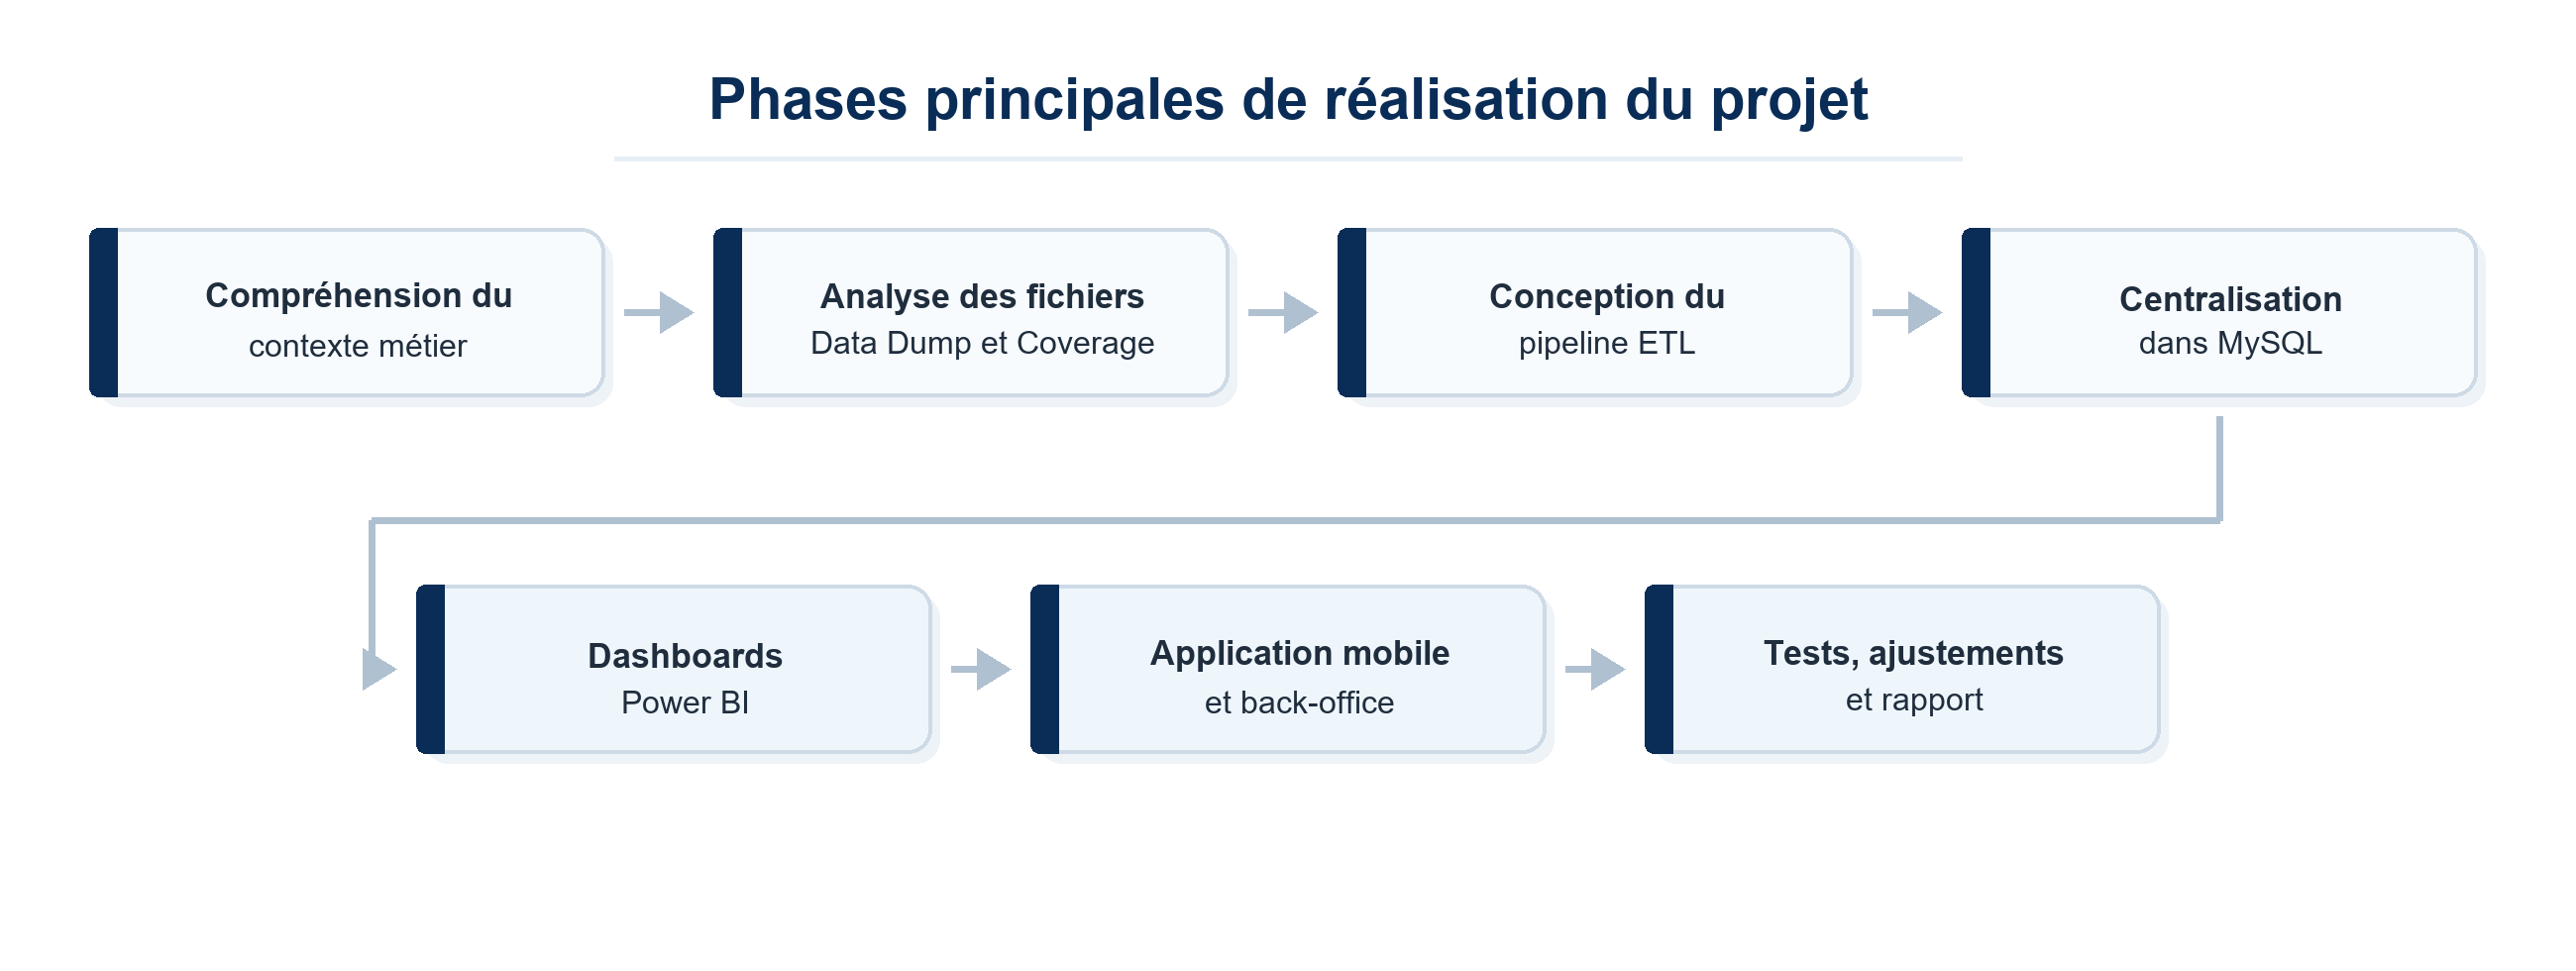
\includegraphics[width=0.95\textwidth]{figures/architecture/project_phases.png}
    \caption{Phases principales de réalisation du projet}
    \label{fig:project-phases}
\end{figure}

Cette organisation met en évidence la logique de progression adoptée. Les premières phases ont permis de comprendre le besoin et de structurer les données, tandis que les phases suivantes ont porté sur la restitution, les interfaces de consultation et les ajustements nécessaires à partir des résultats observés.

\subsection{Planification du projet}

La planification du projet doit permettre de situer les principales étapes de travail dans le temps. Elle repose sur une progression structurée depuis le cadrage métier jusqu’aux tests et à la rédaction du rapport.

La figure suivante accompagne la présentation de la planification générale du projet.

\begin{figure}[H]
    \centering
    
\includegraphics[width=0.45\textwidth]{SMOLLAN.png}
    \caption{Illustration de la planification générale du projet}
    \label{fig:gantt-pfe}
\end{figure}

La planification du projet couvre les principales étapes de réalisation, depuis la compréhension du contexte métier jusqu’aux tests et à la rédaction du rapport. Elle inclut notamment l’analyse des fichiers Data Dump et Coverage, la conception du pipeline ETL, la centralisation des données, la réalisation des tableaux de bord, le développement des interfaces applicatives et les ajustements réalisés au cours du stage.

\section{Conclusion}

Ce chapitre a présenté le cadre général du Projet de Fin d’Études, en introduisant l’organisme d’accueil, le client Unilever ainsi que le contexte métier du merchandising terrain. Il a également permis de formuler la problématique du projet et de préciser les objectifs poursuivis.

Le projet s’inscrit dans une démarche de valorisation des données terrain, visant à mieux structurer les informations issues des opérations de merchandising et à proposer des outils adaptés aux besoins des différents utilisateurs. Le chapitre suivant sera consacré à l’analyse de l’existant et des besoins, afin de détailler le fonctionnement actuel du processus et les limites qui justifient la solution proposée.

\chapter{État de l’existant et cadre théorique}

\section{Introduction}

Ce chapitre présente l’état de l’existant relatif au suivi des opérations terrain du projet Unilever. Il décrit le fonctionnement actuel du processus de reporting, les principales sources de données exploitées, ainsi que les rapports produits à partir des exports issus de la plateforme Smollan.

Il introduit également les notions métier et techniques nécessaires à la compréhension du projet. Ainsi, le chapitre joue un double rôle : présenter l’information existante dans son contexte opérationnel et clarifier les concepts liés au merchandising terrain, aux indicateurs de suivi et à l’exploitation des données.

L’objectif est d’identifier les limites du fonctionnement actuel et de dégager les besoins fonctionnels et techniques auxquels la solution proposée doit répondre. Cette analyse constitue une étape essentielle avant la conception de l’architecture globale du projet.

\section{Cadre théorique du projet}

\subsection{Merchandising terrain et exécution en point de vente}

Le merchandising terrain désigne l’ensemble des actions réalisées en magasin afin d’assurer une bonne présentation des produits et une exécution conforme aux standards définis. Il concerne notamment la disponibilité des produits, leur visibilité en rayon, leur placement, la qualité d’exécution et le respect des consignes commerciales.

Dans le cadre des opérations suivies par Smollan, ces actions sont réalisées par des merchandisers lors des visites en point de vente. Les informations collectées peuvent inclure les réponses aux tâches, les photos justificatives, les relevés liés aux produits, les données de localisation et les éléments nécessaires au reporting. Ces données permettent de vérifier l’état réel de l’exécution terrain et d’alimenter les analyses opérationnelles.

\subsection{Indicateurs de suivi opérationnel}

Le pilotage des opérations de merchandising repose sur plusieurs indicateurs permettant de mesurer l’avancement des visites et la qualité de l’exécution. La couverture permet de suivre les magasins planifiés, visités ou non visités. Les visites exécutées indiquent les interventions effectivement réalisées, tandis que les déviations et les visites rejetées signalent des situations nécessitant une vérification ou une action de suivi.

D’autres indicateurs concernent directement l’exécution commerciale en magasin. L’OSA permet d’évaluer la disponibilité des produits en rayon. Le SOS (\textit{Share of Shelf}) mesure la part de linéaire occupée par une marque ou une catégorie. La qualité d’exécution et le respect du planogramme permettent de vérifier si les produits sont présentés conformément aux standards attendus. Ces indicateurs sont complémentaires, car ils permettent d’analyser à la fois l’avancement terrain et la qualité des actions réalisées.

\subsection{Exploitation des données terrain}

Les données terrain ne peuvent pas être exploitées efficacement lorsqu’elles restent dispersées dans plusieurs fichiers ou rapports séparés. Avant leur utilisation dans des tableaux de bord, une application mobile ou un portail back-office, elles doivent être nettoyées, structurées et centralisées dans un modèle cohérent.

Cette centralisation permet de conserver un historique exploitable, de rapprocher les informations issues de différentes sources et de produire des indicateurs fiables. Elle facilite également la distinction entre les usages internes et les usages orientés client. Les tableaux de bord servent au pilotage et à l’analyse, l’application mobile permet une consultation ciblée des informations par les superviseurs concernés, tandis que le portail back-office reste destiné aux validations et contrôles internes.

Après avoir présenté ces notions générales, il convient d’analyser le fonctionnement actuel du suivi opérationnel afin d’identifier les limites auxquelles la solution proposée doit répondre.
\section{Processus actuel de suivi opérationnel}

Dans le cadre du projet Unilever, le suivi des activités terrain repose initialement sur les données issues de la plateforme opérationnelle utilisée par Smollan. Les merchandisers réalisent leurs visites à travers l’application terrain, dans laquelle ils renseignent les informations liées à l’exécution en magasin : présence au point de vente, tâches réalisées, réponses aux questionnaires, disponibilité des produits, éléments de qualité, photos justificatives et données de localisation.

Le processus actuel s’appuie principalement sur l’extraction quotidienne de fichiers Excel depuis la plateforme Smollan. Ces exports permettent de suivre l’activité de la veille ou d’une période sélectionnée. Les deux fichiers les plus importants dans ce processus sont le fichier \textit{Data Dump} et le fichier \textit{Coverage}. Le premier regroupe les détails d’exécution saisis sur le terrain, tandis que le second apporte une vision plus opérationnelle de la couverture, des visites planifiées, des visites réalisées, des visites adhoc, des rejets, des déviations et des magasins non visités.

Ces fichiers sont exploités pour produire différents reportings. Certains sont orientés vers le suivi interne, notamment les rapports de couverture, de déviation, de visites rejetées et de magasins non visités. D’autres sont destinés au client Unilever, comme le suivi OSA transmis quotidiennement, ainsi que des reportings plus spécifiques ou périodiques liés à la qualité d’exécution, au SOS, au placement en rayon ou à d’autres indicateurs terrain. Ces reportings permettent de suivre l’état d’avancement des opérations, d’analyser la disponibilité des produits, d’identifier les magasins nécessitant un suivi particulier et de faciliter les actions de suivi.

Ce processus permet d’assurer un suivi quotidien des opérations. Toutefois, il reste fortement dépendant des exports Excel et de traitements séparés. Les informations nécessaires à l’analyse sont présentes, mais elles sont dispersées entre plusieurs fichiers et rapports. De plus, le fichier Data Dump ne suffit pas à lui seul pour reconstituer toute la situation opérationnelle, car certaines informations liées aux visites planifiées, non réalisées ou rejetées sont principalement disponibles dans le fichier Coverage. Cette situation rend plus difficile la constitution d’un historique structuré, l’accès rapide aux détails d’exécution d’un magasin et la mise en place d’indicateurs consolidés pour le pilotage opérationnel.


La figure suivante présente une vue simplifiée du processus actuel de reporting, depuis la saisie des informations terrain dans l'application Smart 3 jusqu'à la production des rapports internes et des reportings destinés au client Unilever.

\begin{figure}[H]
    \centering
    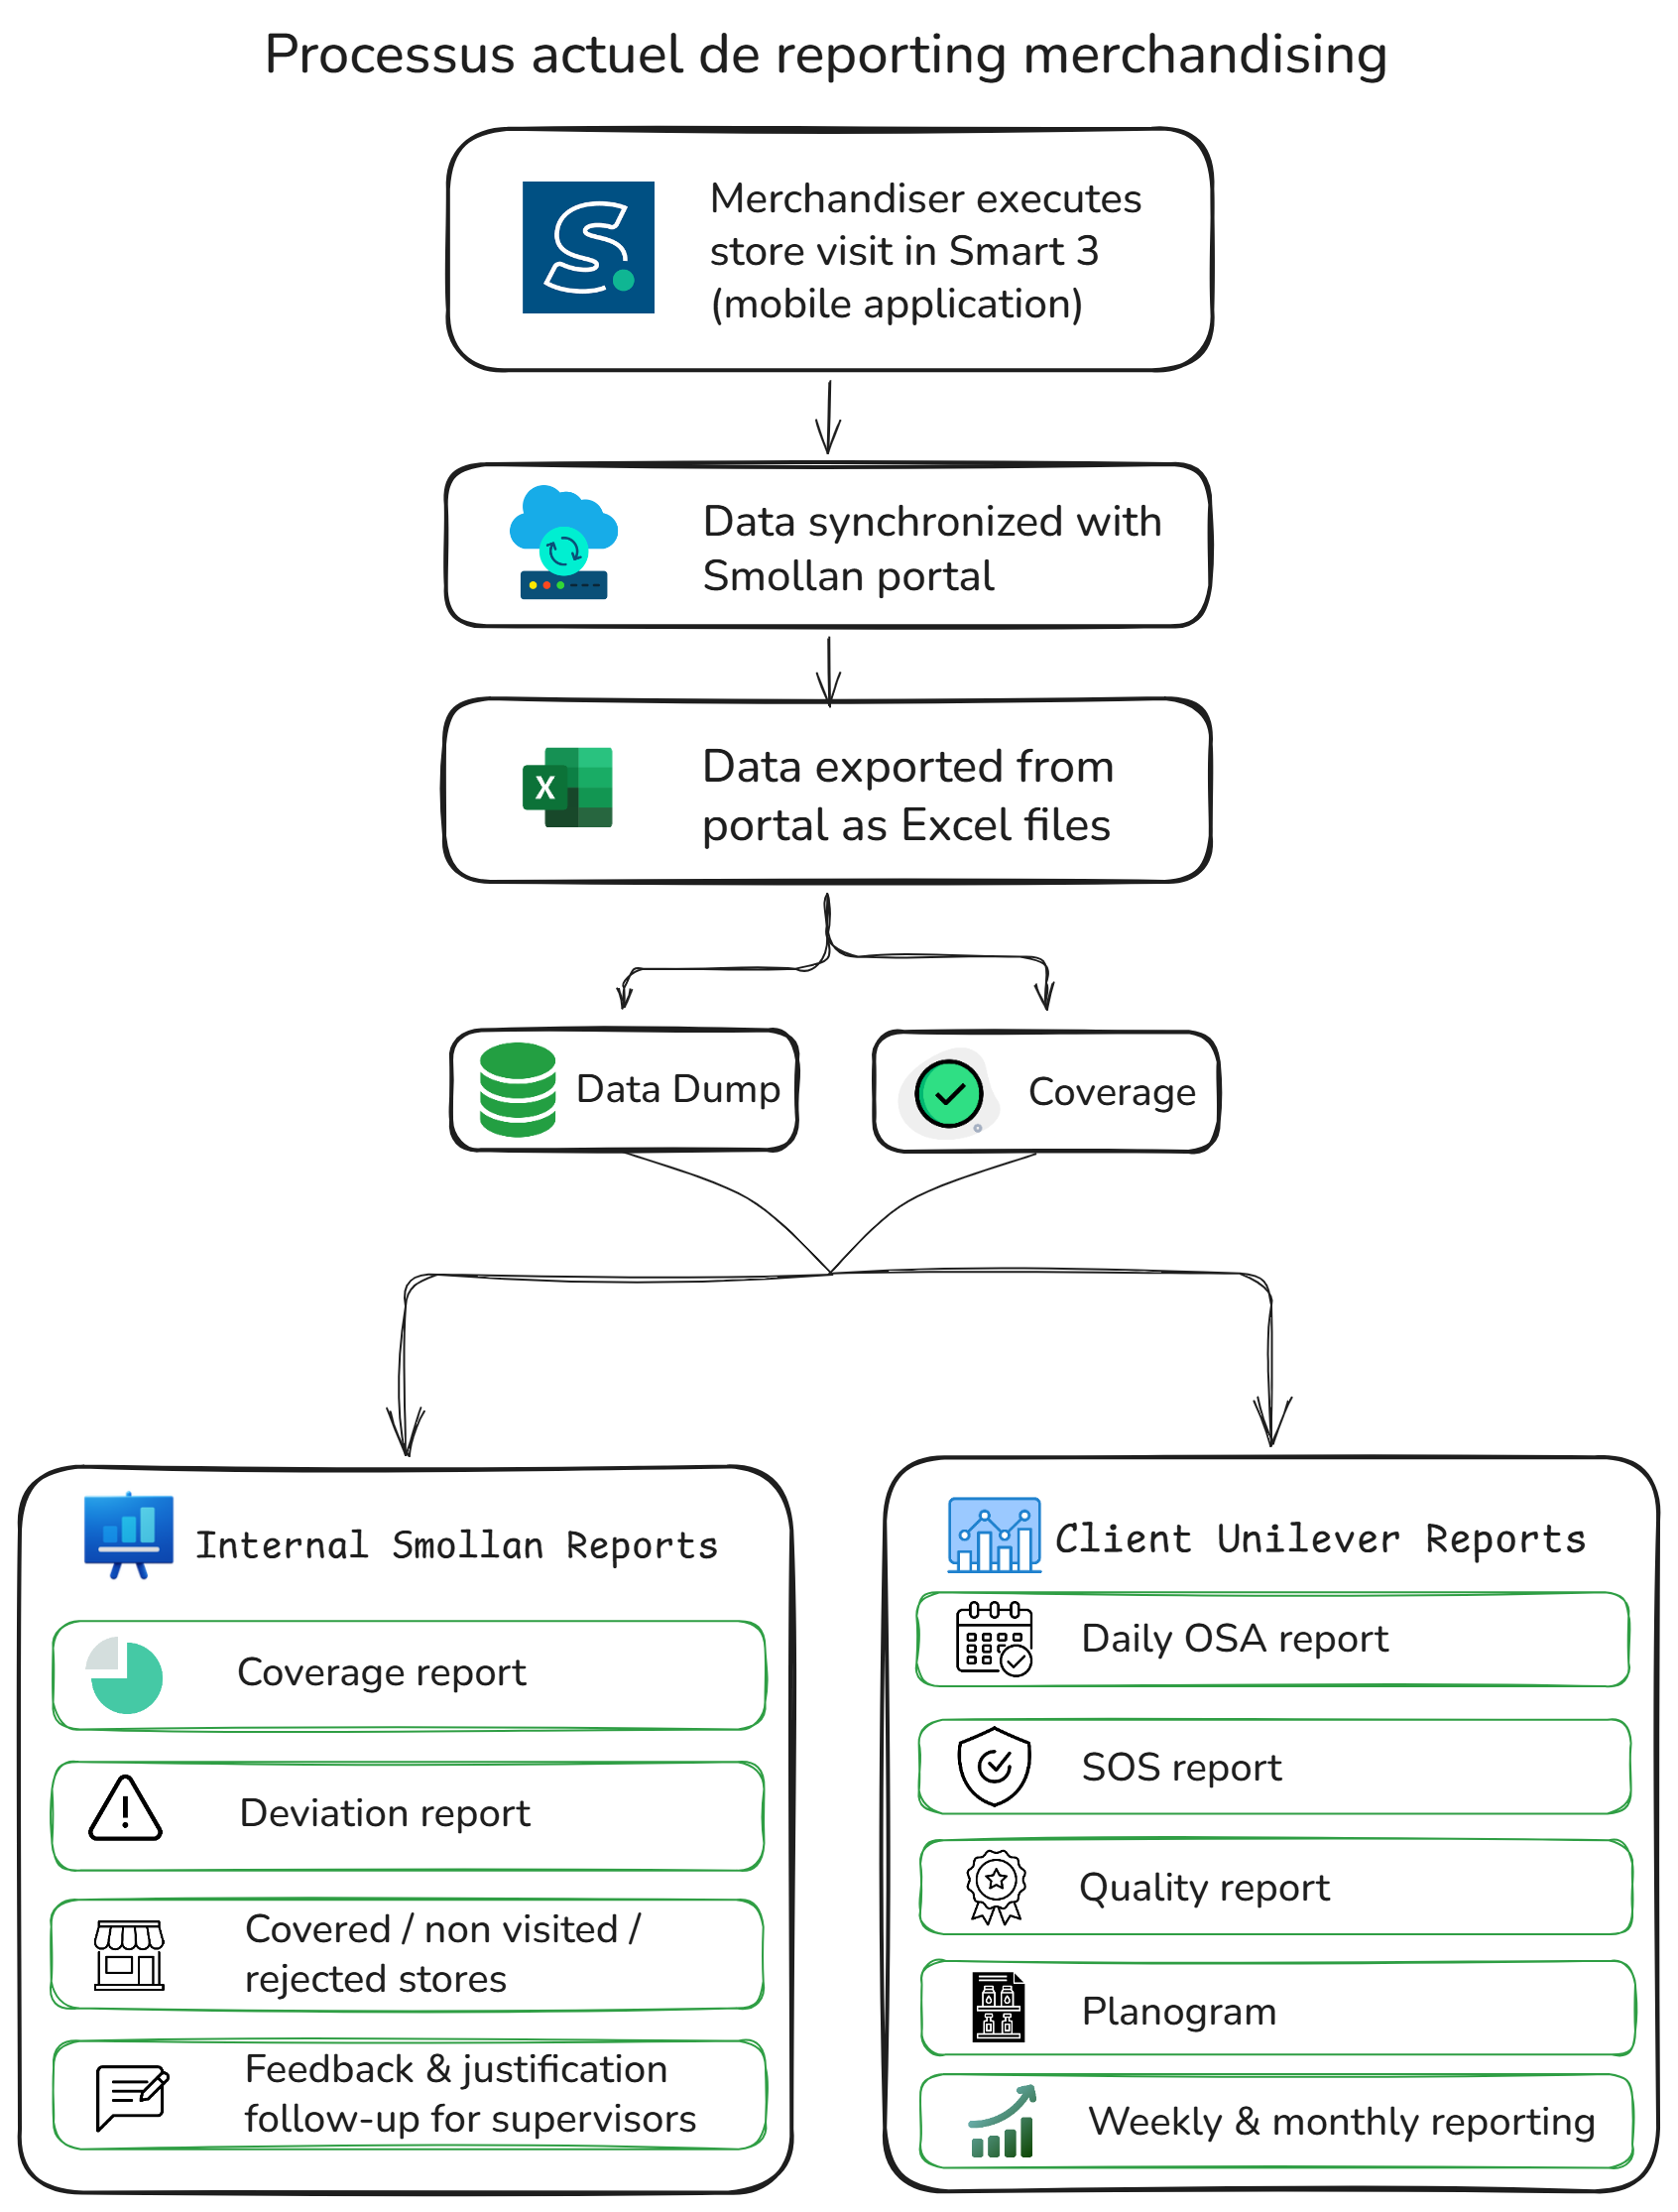
\includegraphics[width=0.85\textwidth]{figures/architecture/Processus_actuel_de_suivi_opérationnel.png}
    \caption{Processus actuel de reporting merchandising basé sur Smart 3 et les exports Excel}
    \label{fig:current-reporting-process}
\end{figure}

Cette figure montre que les exports issus du portail Smollan constituent le point de départ de plusieurs usages. Les rapports internes sont principalement orientés vers le suivi opérationnel, notamment la couverture, les déviations, les rejets et les justifications terrain. Les reportings destinés au client Unilever sont davantage orientés vers la disponibilité produit, la qualité d’exécution, le SOS, le planogramme et les analyses hebdomadaires ou mensuelles.

\section{Sources de données exploitées}

\subsection{Fichier Data Dump}

Le fichier \textit{Data Dump} constitue la source principale des données détaillées issues de l’exécution terrain. Il contient les réponses renseignées par les merchandisers lors de leurs visites en magasin, ainsi que les informations associées aux tâches exécutées.

Ce fichier regroupe notamment les données relatives aux merchandisers, aux magasins, aux produits, aux catégories, aux tâches, aux questions posées et aux réponses saisies. Il contient également des informations liées aux dates d’exécution, aux coordonnées de localisation collectées par l’application terrain et, dans certains cas, aux liens vers les photos justificatives.

Dans le cadre du projet, le \textit{Data Dump} permet d’analyser plusieurs dimensions de l’exécution merchandising, telles que l’OSA, la qualité d’exécution, le placement primaire, le placement secondaire, le SOS, les relevés de prix, les conditions magasin ainsi que les opérations de check-in et check-out. Il représente donc une source riche pour comprendre ce qui a été réellement renseigné sur le terrain.

Toutefois, cette richesse s’accompagne d’une certaine complexité. Les données sont organisées sous forme de lignes de réponses, avec des tâches, des questions et des formats variables selon les cas. Cette structure nécessite un traitement de transformation afin de construire des tables exploitables pour l’analyse, la validation et la restitution dans les tableaux de bord.

\subsection{Fichier Coverage}

Le fichier \textit{Coverage} apporte une vision plus synthétique et opérationnelle de l’activité terrain. Contrairement au \textit{Data Dump}, qui décrit principalement les réponses et les tâches renseignées lors des visites, le fichier \textit{Coverage} permet de suivre l’état des visites prévues et réalisées.

Il contient notamment les informations liées aux visites planifiées, aux visites exécutées, aux visites adhoc, aux visites rejetées, aux déviations, aux magasins non visités, aux merchandisers, aux superviseurs, aux formats de magasins, aux villes, aux régions, ainsi qu’à certaines informations de durée et de localisation.

Ce fichier est essentiel pour le calcul des indicateurs opérationnels, notamment le taux de couverture, le nombre de visites exécutées, les visites non réalisées, les rejets, les déviations et l’activité des merchandisers sur une période donnée. Il permet également d’alimenter les vues de suivi utilisées dans les tableaux de bord et dans l’application mobile.

Ainsi, le fichier \textit{Coverage} joue un rôle central dans la compréhension de l’état d’avancement du terrain, car il permet de relier la planification des visites à leur réalisation effective.

\subsection{Complémentarité Data Dump / Coverage}

Les fichiers \textit{Data Dump} et \textit{Coverage} sont complémentaires. Le \textit{Data Dump} permet d’analyser le contenu détaillé des visites exécutées, tandis que le \textit{Coverage} permet de reconstituer la vision opérationnelle globale des visites planifiées, réalisées, rejetées ou non effectuées.

Cette complémentarité est importante, car l’analyse de l’exécution terrain ne peut pas reposer uniquement sur les réponses détaillées des tâches. Par exemple, un magasin non visité ou une visite rejetée peut ne pas disposer du même niveau de détail dans le \textit{Data Dump}, alors que ces informations sont indispensables pour le suivi opérationnel. Le fichier \textit{Coverage} permet donc de compléter cette lecture en apportant le statut des visites et les informations de couverture.

Dans le cadre de la solution développée, l’exploitation conjointe de ces deux sources permet de construire une base de données plus cohérente. Les données détaillées issues du \textit{Data Dump} alimentent les tables de tâches et les réponses normalisées, tandis que les données du \textit{Coverage} alimentent les indicateurs de suivi opérationnel. Cette approche permet d’obtenir une vision à la fois détaillée et globale des activités terrain.


Le tableau suivant synthétise le rôle de chaque source dans la solution proposée.

\begin{table}[H]
\centering
\caption{Comparaison entre les fichiers Data Dump et Coverage}
\label{tab:data-dump-coverage}
\renewcommand{\arraystretch}{1.25}
\small
\begin{tabular}{
|>{\raggedright\arraybackslash}p{2.8cm}
|>{\raggedright\arraybackslash}p{4cm}
|>{\raggedright\arraybackslash}p{4cm}
|>{\raggedright\arraybackslash}p{4cm}|
}
\hline
\textbf{Fichier} & \textbf{Type d'information} & \textbf{Utilité dans le projet} & \textbf{Limite principale} \\
\hline
\textit{Data Dump}
& Données détaillées d'exécution terrain : tâches, questions, réponses, produits, photos et informations de localisation.
& Analyse du contenu des visites réalisées : réponses OSA, qualité d'exécution, placement en rayon, SOS et autres tâches terrain.
& Ne permet pas à lui seul de reconstituer toute la situation opérationnelle, notamment les visites non réalisées ou certains statuts de couverture. \\
\hline
\textit{Coverage}
& Données de suivi opérationnel : visites planifiées, visites réalisées, visites adhoc, rejets, déviations, magasins non visités et informations de supervision.
& Calcul des KPI de couverture, suivi de l'avancement terrain et alimentation des vues de pilotage opérationnel.
& Ne fournit pas toujours le détail complet des réponses terrain et des tâches exécutées, principalement disponibles dans le \textit{Data Dump}. \\
\hline
\end{tabular}
\end{table}

Cette comparaison montre que les deux fichiers répondent à des besoins différents. Le \textit{Data Dump} apporte le détail de l'exécution terrain, tandis que le \textit{Coverage} permet de suivre l'état global des visites. Leur combinaison constitue donc une base nécessaire pour construire une lecture fiable des opérations.


\section{Rapports existants}

Les fichiers exportés depuis la plateforme Smollan servent de base à plusieurs reportings utilisés dans le suivi des opérations terrain. Ces reportings peuvent être regroupés en deux grandes catégories : les rapports destinés au suivi interne des opérations et les rapports destinés au client Unilever.

\subsection{Rapports internes Smollan}

Les rapports internes sont principalement orientés vers le suivi opérationnel quotidien. Ils permettent de suivre l’état de couverture, les visites réalisées, les visites non effectuées, les déviations, les rejets et certains éléments liés à l’assiduité ou au temps de production. Ces rapports facilitent la lecture de l’activité terrain et permettent d’identifier les situations nécessitant un suivi opérationnel.

Parmi les rapports internes les plus utilisés, on retrouve notamment les rapports de couverture et les rapports de déviation. Le rapport de couverture permet d’obtenir une vision de l’avancement des visites, tandis que le rapport de déviation met en évidence les magasins nécessitant une confirmation, une justification ou une revisite selon le contexte terrain.

Ces reportings jouent donc un rôle important dans la coordination quotidienne des opérations. Toutefois, ils restent généralement produits sous forme de fichiers séparés, ce qui limite l’analyse historique et la centralisation des informations dans une seule base exploitable.

\subsection{Rapports destinés au client Unilever}

En parallèle des rapports internes, certaines restitutions sont destinées au client Unilever. Elles concernent principalement la qualité d’exécution en magasin, la disponibilité des produits et certains indicateurs liés à la visibilité ou à la présence des produits en rayon.

Le suivi OSA constitue un exemple important de reporting client, car il permet d’analyser la disponibilité des produits dans les magasins visités. D’autres reportings, comme les rapports liés à la qualité d’exécution, au SOS, au placement en rayon ou à d’autres indicateurs terrain, peuvent être produits de manière périodique ou selon les besoins du suivi opérationnel.

Ces rapports permettent au client de disposer d’une lecture sur l’exécution terrain et sur les points nécessitant une attention particulière. Cependant, comme pour les rapports internes, leur exploitation reste dépendante des fichiers sources et des traitements réalisés en amont.

Le tableau suivant résume les principaux types de reportings produits à partir des fichiers opérationnels.

\begin{table}[H]
\centering
\caption{Synthèse des reportings existants}
\label{tab:reportings-existants}
\renewcommand{\arraystretch}{1.25}
\small
\begin{tabular}{
|>{\raggedright\arraybackslash}p{3.2cm}
|>{\raggedright\arraybackslash}p{3.2cm}
|>{\raggedright\arraybackslash}p{3cm}
|>{\raggedright\arraybackslash}p{5cm}|
}
\hline
\textbf{Type de rapport} & \textbf{Destinataire} & \textbf{Fréquence} & \textbf{Objectif principal} \\
\hline
Rapport de couverture
& Suivi interne
& Quotidienne
& Suivre l’avancement des visites, les magasins couverts, les magasins non visités et l’état global du terrain. \\
\hline
Rapport de déviation
& Suivi interne
& Quotidienne ou selon le besoin
& Identifier les magasins nécessitant une confirmation, une justification ou une action de suivi. \\
\hline
Suivi OSA
& Client Unilever
& Quotidienne
& Suivre la disponibilité des produits et identifier les références non disponibles en magasin. \\
\hline
Rapports qualité, SOS et placement
& Client Unilever
& Périodique ou selon le besoin
& Analyser la qualité d’exécution, la présence produit, le placement en rayon et les points nécessitant une attention particulière. \\
\hline
\end{tabular}
\end{table}

Ce tableau montre que les reportings existants répondent à des besoins complémentaires. Les rapports internes soutiennent le pilotage quotidien des opérations, tandis que les reportings destinés au client permettent de suivre la disponibilité, la qualité d’exécution et la visibilité des produits en magasin.

\section{Limites du processus actuel}

Le processus actuel permet d'assurer un suivi quotidien des opérations terrain, mais il présente plusieurs limites lorsque les volumes de données augmentent et lorsque les besoins d'analyse deviennent plus avancés. La première limite concerne la dépendance aux fichiers Excel exportés depuis la plateforme. Ces fichiers restent indispensables au suivi opérationnel, mais leur exploitation sous forme de rapports séparés rend plus difficile la centralisation de l'information et la construction d'une vision historique consolidée.

La deuxième limite concerne la dispersion des données entre plusieurs sources. Le fichier \textit{Data Dump} contient les détails d'exécution, tandis que le fichier \textit{Coverage} apporte les informations de couverture et de statut des visites. Cette complémentarité est nécessaire, mais elle impose un travail de rapprochement afin de produire des indicateurs fiables. Sans modèle de données centralisé, l'analyse peut devenir répétitive et dépendante de traitements manuels ou semi-automatisés.

Une autre limite concerne l'accès aux détails d'exécution par magasin. Les rapports existants permettent de suivre l'état global des opérations, mais l'accès rapide à l'historique d'un magasin, aux tâches exécutées, aux réponses terrain ou aux éléments justificatifs reste moins direct. Cette situation limite la capacité à consulter facilement une vision détaillée et structurée de l'exécution terrain.

Enfin, les besoins de suivi ne sont pas identiques selon les utilisateurs. Les équipes internes ont besoin d'indicateurs de pilotage, de contrôle et de validation opérationnelle, tandis que les superviseurs côté client doivent disposer d'une consultation plus ciblée sur les magasins qui leur sont affectés. Cette différence d'usage montre la nécessité de distinguer les couches de restitution : tableaux de bord BI pour le pilotage, application mobile client pour la consultation des magasins affectés, et portail back-office pour le suivi interne des validations.

\section{Besoins fonctionnels}

À partir des limites identifiées dans le processus actuel, plusieurs besoins fonctionnels ont été définis afin de structurer la solution proposée. Ces besoins concernent à la fois la centralisation des données, le suivi des indicateurs opérationnels, la consultation des informations terrain et la validation interne des situations nécessitant une analyse complémentaire.

Le premier besoin consiste à mettre en place une base de données centralisée capable de regrouper les informations issues des fichiers \textit{Data Dump} et \textit{Coverage}. Cette base doit permettre de conserver l'historique des données, de structurer les informations relatives aux visites, aux magasins, aux merchandisers, aux produits et aux tâches exécutées, et de faciliter leur exploitation dans les différentes couches de la solution.

Le deuxième besoin concerne la mise à disposition de tableaux de bord décisionnels permettant de suivre l’avancement des opérations terrain et d’analyser les principaux indicateurs avant la restitution finale. Ces dashboards doivent aider au pilotage interne et au management, tout en facilitant la lecture des données liées à la couverture, à l’activité des merchandisers et à certains reportings client comme l’OSA, la qualité d’exécution, le SOS ou le placement en rayon.

Le troisième besoin concerne le développement d'une application mobile orientée client. Cette application doit permettre aux superviseurs côté Unilever de se connecter et de consulter uniquement les magasins qui leur sont affectés. L'objectif est de leur offrir une visibilité simple et ciblée sur l'exécution terrain, les informations des magasins, les dernières visites et les détails liés aux tâches exécutées.

Le quatrième besoin porte sur la mise en place d'un portail back-office interne destiné au suivi des validations opérationnelles. Ce portail doit permettre d'exploiter les résultats des règles de validation, notamment les cas liés à l'OSA, aux contrôles GPS ou à d'autres situations nécessitant une vérification. Il doit constituer un espace interne de consultation, d'analyse et, à terme, de suivi des actions correctives.

Ainsi, les besoins fonctionnels du projet ne se limitent pas à la production de tableaux de bord. Ils couvrent l'ensemble de la chaîne d'exploitation de la donnée, depuis l'ingestion des fichiers jusqu'à la restitution des informations sous forme de dashboards, d'application mobile client et de portail de validation interne.


\section{Besoins techniques}

La mise en œuvre de la solution nécessite une architecture technique capable de traiter des fichiers Excel volumineux, de structurer les données et de les rendre exploitables par plusieurs outils. Le premier besoin technique concerne la mise en place d’un pipeline ETL développé en Python, permettant d’extraire, nettoyer, transformer et charger les données issues des fichiers \textit{Data Dump} et \textit{Coverage}.

Le deuxième besoin concerne la centralisation des données dans une base MySQL. Cette base doit permettre de stocker les informations opérationnelles, les réponses terrain, les tables liées aux différentes tâches, ainsi que les indicateurs nécessaires aux tableaux de bord, à l’application mobile et au portail de validation.

Le troisième besoin porte sur la restitution et l’intégration des données. Les tableaux de bord sont réalisés avec Power BI afin de faciliter l’analyse et le pilotage des indicateurs. L’application mobile client et le portail back-office nécessitent une couche backend exposant des APIs, développée avec Spring Boot, afin de communiquer avec la base de données et de fournir les informations aux interfaces React.

Enfin, la solution doit rester évolutive afin de permettre l’ajout progressif de nouvelles règles de validation, de nouvelles vues analytiques, de nouveaux fichiers sources comme les Masters, ainsi que des mécanismes d’authentification et de gestion des rôles plus avancés.

\section{Conclusion}

Ce chapitre a permis d’introduire les notions nécessaires à la compréhension du projet, notamment le merchandising terrain, les indicateurs de suivi opérationnel et l’exploitation structurée des données collectées en magasin. Ces éléments théoriques ont posé le cadre métier et technique dans lequel s’inscrit la solution proposée.

L’état de l’existant a ensuite permis d’analyser le fonctionnement actuel du suivi des opérations terrain dans le cadre du projet Unilever. L’étude du processus actuel a montré que les fichiers \textit{Data Dump} et \textit{Coverage} constituent deux sources complémentaires : le premier apporte le détail de l’exécution terrain, tandis que le second permet de suivre la couverture et le statut opérationnel des visites.

L’analyse des rapports existants a également mis en évidence la diversité des usages des données, entre le suivi interne des opérations et les reportings destinés au client Unilever. Malgré l’utilité de ce fonctionnement, plusieurs limites ont été identifiées, notamment la dépendance aux fichiers Excel, la dispersion des informations, la difficulté de constituer un historique centralisé et la nécessité d’adapter les restitutions selon les utilisateurs.

Ces constats ont permis de définir les principaux besoins fonctionnels et techniques du projet. Ils justifient la mise en place d’une solution data-driven reposant sur une base de données centralisée, des tableaux de bord décisionnels, une application mobile client et un portail back-office de validation interne. Le chapitre suivant présentera la conception globale de cette solution ainsi que son architecture fonctionnelle et technique.

\chapter{Conception globale de la solution}

\section{Introduction}
% TODO: Introduire la vision globale avant les chapitres techniques detailles.

\section{Vision generale de la solution}
% TODO: Presenter la solution comme une architecture data-driven en quatre couches.

\section{Architecture globale}
\begin{figure}[htbp]
    \centering
    \fbox{\parbox{0.82\textwidth}{\centering Espace reserve au schema d'architecture globale de la solution.}}
    \caption{Architecture globale de la solution data-driven}
    \label{fig:architecture_globale}
\end{figure}

\section{Separation des couches fonctionnelles}

\subsection{Couche Data Engineering}
% TODO: Presenter le role de l'ETL, de MySQL, de fact_coverage et de survey_responses.

\subsection{Couche Business Intelligence}
% TODO: Presenter le role des dashboards Power BI pour le management et les equipes internes.

\subsection{Couche application mobile client}
% TODO: Presenter l'application mobile comme interface client Unilever orientee magasins affectes.

\subsection{Couche back-office validation interne}
% TODO: Presenter le portail interne Smollan pour les anomalies et la validation.

\section{Choix technologiques}
% TODO: Justifier les choix Python, MySQL, Power BI, Spring Boot, React et Docker.

\section{Conclusion}
% TODO: Faire la transition vers le pipeline Data Engineering.


\chapter{Mise en place du pipeline Data Engineering}

\section{Introduction}
% TODO: Introduire le role du pipeline Data Engineering dans la solution.

\section{Ingestion des fichiers Excel}
% TODO: Decrire l'ingestion des fichiers Data Dump et Coverage.

\section{Traitement du Data Dump}
% TODO: Presenter les transformations principales liees aux visites, taches et reponses terrain.

\section{Traitement du Coverage}
% TODO: Presenter le role de fact_coverage pour la couverture, les statuts et les KPI.

\section{Modelisation et chargement dans MySQL}
% TODO: Decrire les tables principales et les relations utiles.

\begin{figure}[htbp]
    \centering
    \fbox{\parbox{0.82\textwidth}{\centering Espace reserve au diagramme du flux ETL.}}
    \caption{Flux general du pipeline ETL}
    \label{fig:flux_etl}
\end{figure}

\section{Tables dynamiques par tache}
% TODO: Expliquer le principe des tables task_* et leurs limites.

\section{Table normalisee survey\_responses}
% TODO: Expliquer pourquoi survey_responses facilite l'analyse et la validation.

\section{Integration future des Masters}
% TODO: Presenter les Masters comme extension future pour les dimensions de planification.

\section{Conclusion}
% TODO: Faire la transition vers la couche Business Intelligence.


\chapter{Business Intelligence et tableaux de bord operationnels}

\section{Introduction}
% TODO: Introduire le role de Power BI dans le pilotage operationnel.

\section{Objectifs des dashboards}
% TODO: Expliquer les objectifs management, boss et field team.

\section{Definition des KPI operationnels}
% TODO: Decrire les KPI reels utilises sans inventer de resultats.

\section{Dashboard executif}
\begin{figure}[htbp]
    \centering
    \fbox{\parbox{0.82\textwidth}{\centering Espace reserve a la capture du dashboard executif Power BI.}}
    \caption{Dashboard executif de suivi operationnel}
    \label{fig:dashboard_executif}
\end{figure}

\section{Dashboard Merchandiser Performance Intelligence}
\begin{figure}[htbp]
    \centering
    \fbox{\parbox{0.82\textwidth}{\centering Espace reserve a la capture du dashboard Merchandiser Performance Intelligence.}}
    \caption{Dashboard d'analyse de performance des merchandisers}
    \label{fig:dashboard_merch}
\end{figure}

\section{Analyse GT / MT}
% TODO: Presenter l'analyse GT/MT et son interet business.

\section{Apport pour le management et le field team}
% TODO: Expliquer l'apport des dashboards pour les decisions operationnelles.

\section{Conclusion}
% TODO: Faire la transition vers l'application mobile client.


\chapter{Application mobile client pour le suivi des magasins affectes}

\section{Introduction}
% TODO: Introduire le changement de scope vers une application client Unilever.

\section{Objectif de l'application mobile client}
% TODO: Presenter l'objectif client-facing de l'application.

\section{Logique d'acces par superviseur client}
% TODO: Expliquer la logique d'acces par compte superviseur client.

\section{Filtrage des magasins par store\_code}
% TODO: Decrire le filtrage des magasins affectes par store_code.

\section{Module Dashboard client}
% TODO: Presenter uniquement les indicateurs adaptes au client.

\section{Module Stores}
% TODO: Presenter la vue map/list des magasins affectes.

\section{Detail d'execution d'un magasin}
% TODO: Presenter les informations client-safe affichees dans le detail magasin.

\section{Limites actuelles de l'application}
% TODO: Mentionner les limites sans exposer de resultats non finalises.

\section{Conclusion}
% TODO: Faire la transition vers le portail back-office interne.


\chapter{Portail back-office de validation interne}

\section{Introduction}
% TODO: Introduire le role interne du portail back-office pour Smollan.

\section{Objectif du portail de validation}
% TODO: Expliquer que ce portail porte les controles internes et le suivi des anomalies.

\section{Moteur de regles de validation}
% TODO: Presenter le moteur Python et les regles enregistrees.

\section{Tables validation\_run\_log et validation\_results}
% TODO: Decrire la tracabilite des executions et des anomalies detectees.

\section{Suivi des anomalies OSA et GPS}
% TODO: Presenter les regles OSA et GPS sans exagerer leur maturite.

\section{Dashboard de validation existant}
\begin{figure}[htbp]
    \centering
    \fbox{\parbox{0.82\textwidth}{\centering Espace reserve a la capture du portail back-office de validation.}}
    \caption{Dashboard interne de validation}
    \label{fig:dashboard_validation}
\end{figure}

\section{Workflow de validation prevu}
% TODO: Presenter comme perspective : pending/reviewed, commentaires, action needed, reviewed_by, reviewed_at.

\section{Conclusion}
% TODO: Faire la transition vers les resultats, limites et perspectives.


\chapter{Resultats, limites et perspectives}

\section{Introduction}
% TODO: Introduire le bilan du projet.

\section{Resultats obtenus}
% TODO: Presenter uniquement les resultats reels et verifies.

\section{Apports du projet}
% TODO: Distinguer les apports data, BI, mobile client et back-office interne.

\section{Limites actuelles}
% TODO: Presenter les limites avec transparence.

\section{Perspectives}

\subsection{Integration complete des Masters}
% TODO: Presenter l'integration des Masters comme evolution future.

\subsection{Authentification et gestion des roles}
% TODO: Presenter le besoin de renforcer les acces et les roles.

\subsection{Workflow complet de validation}
% TODO: Presenter le workflow interne cible.

\subsection{Orchestration des pipelines}
% TODO: Presenter Airflow ou Prefect comme perspective.

\subsection{Machine Learning et detection avancee d'anomalies}
% TODO: Presenter cette piste comme perspective, sans annoncer une realisation.

\section{Conclusion}
% TODO: Conclure le chapitre.


\chapter*{Conclusion generale}
\addcontentsline{toc}{chapter}{Conclusion generale}

% TODO: Rediger la conclusion generale apres finalisation des chapitres.
% Elle devra synthetiser les apports reels du projet, ses limites et les perspectives principales.

\section*{Synthese du travail realise}

\section*{Apports du projet}

\section*{Limites et perspectives}

\section*{Conclusion finale}



\clearpage
\chapter*{Bibliographie}
\addcontentsline{toc}{chapter}{Bibliographie}
% TODO: Ajouter ici la bibliographie finale ou activer BibTeX avec references.bib.

\appendix
\chapter{Annexes}

\section{Schemas techniques}
% TODO: Ajouter les schemas d'architecture, ETL et base de donnees.

\section{Captures d'ecran}
% TODO: Ajouter les captures Power BI, mobile/web et validation.

\section{Exemples techniques}
% TODO: Ajouter les exemples de requetes SQL, endpoints API ou extraits anonymises.


\end{document}
